\documentclass[11pt,letterpaper]{article}

\usepackage[utf8]{inputenc}
\usepackage[T1]{fontenc}
\usepackage[spanish,es-nodecimaldot]{babel}
\usepackage{lmodern}
\usepackage{microtype}
\usepackage{geometry}
\usepackage{graphicx}
\usepackage{booktabs}
\usepackage{array}
\usepackage{float}
\usepackage{caption}
\usepackage{subcaption}
\usepackage{setspace}
\usepackage[hidelinks]{hyperref}

\geometry{top=2.5cm,bottom=2.5cm,left=2.8cm,right=2.8cm}
\graphicspath{{../outputs/}}
\setstretch{1.12}
\setlength{\parindent}{1.2em}
\setlength{\parskip}{0.25em}
\captionsetup{font=small,labelfont=bf}

% Enlace al video de demostracion.
\newcommand{\videourl}{https://youtu.be/QKezHRry-co}

\title{Clasificaci\'on de se\~nales de tr\'ansito mediante redes neuronales convolucionales}
\author{Mar\'ia Jos\'e Gir\'on -- 23559 \and Leonardo Mej\'ia -- 23648 \and Milton Polanco -- 23471 \and Dilary Cruz -- 231010}
\date{Octubre de 2026}

\begin{document}

\begin{titlepage}
    \centering
    {\large Universidad del Valle de Guatemala\par}
    \vspace{0.5cm}
    {\large CC2017 -- Deep Learning\par}
    \vfill
    {\LARGE\bfseries Clasificaci\'on de se\~nales de tr\'ansito mediante redes neuronales convolucionales\par}
    \vspace{0.8cm}
    {\large Comparaci\'on entre una CNN entrenada desde cero y MobileNetV2\par}
    \vfill
    {\large Mar\'ia Jos\'e Gir\'on -- 23559\par}
    {\large Leonardo Mej\'ia -- 23648\par}
    {\large Milton Polanco -- 23471\par}
    {\large Dilary Cruz -- 231010\par}
    \vfill
    {\large Octubre de 2026\par}
\end{titlepage}

\pagenumbering{roman}
\tableofcontents
\listoffigures
\listoftables
\clearpage
\pagenumbering{arabic}

\begin{abstract}
Este trabajo estudia la clasificaci\'on autom\'atica de se\~nales de tr\'ansito mediante aprendizaje profundo. Se compar\'o una red convolucional compacta entrenada desde cero con MobileNetV2 preentrenada en ImageNet, tanto con el extractor de caracter\'isticas congelado como mediante ajuste fino. Los experimentos emplearon las 43 clases del conjunto German Traffic Sign Recognition Benchmark (GTSRB), con una separaci\'on de entrenamiento y validaci\'on agrupada por secuencia de captura para evitar fuga de datos. La CNN propia obtuvo 99.18\% de exactitud y 98.70\% de F1 macro en el test oficial, mientras que MobileNetV2 alcanz\'o 59.91\% con el backbone congelado y 76.76\% despu\'es del ajuste fino. Tambi\'en se evalu\'o la robustez ante oscurecimiento, ruido gaussiano y desenfoque, y se utilizaron mapas Grad-CAM para analizar las regiones relevantes. Los resultados muestran que la arquitectura compacta especializada supera a los modelos transferidos en este dominio y que el desenfoque intenso constituye su principal debilidad.
\end{abstract}

\section{Descripci\'on del problema}

El reconocimiento de se\~nales de tr\'ansito es un componente de los sistemas avanzados de asistencia al conductor y de la percepci\'on para veh\'iculos aut\'onomos. Un clasificador debe distinguir se\~nales con diferencias sutiles, como los distintos l\'imites de velocidad, bajo variaciones de escala, iluminaci\'on, enfoque y perspectiva. Los errores pueden producirse entre clases visualmente parecidas aun cuando el objeto general haya sido localizado correctamente.

El objetivo del proyecto es construir y evaluar un sistema capaz de asignar una imagen a una de las 43 clases de GTSRB. Adem\'as de medir exactitud, se busca responder cuatro preguntas: (1) si una CNN compacta puede aprender el dominio desde cero; (2) si las caracter\'isticas aprendidas en ImageNet se transfieren a se\~nales de baja resoluci\'on; (3) qu\'e clases y condiciones producen los errores principales; y (4) qu\'e regiones de la imagen sustentan una predicci\'on.

\section{An\'alisis del conjunto de datos}

GTSRB contiene 39,209 im\'agenes de entrenamiento y 12,630 im\'agenes de test distribuidas en 43 clases \cite{stallkamp2012}. Las im\'agenes de entrenamiento tienen anchos entre 25 y 243 p\'ixeles y alturas entre 25 y 225 p\'ixeles. La clase menos frecuente contiene 210 observaciones y la m\'as frecuente 2,250, una raz\'on de 10.7 a 1. Esta variaci\'on justifica reportar F1 macro, que otorga igual peso a cada clase, junto con exactitud y m\'etricas ponderadas.

\begin{figure}[H]
    \centering
    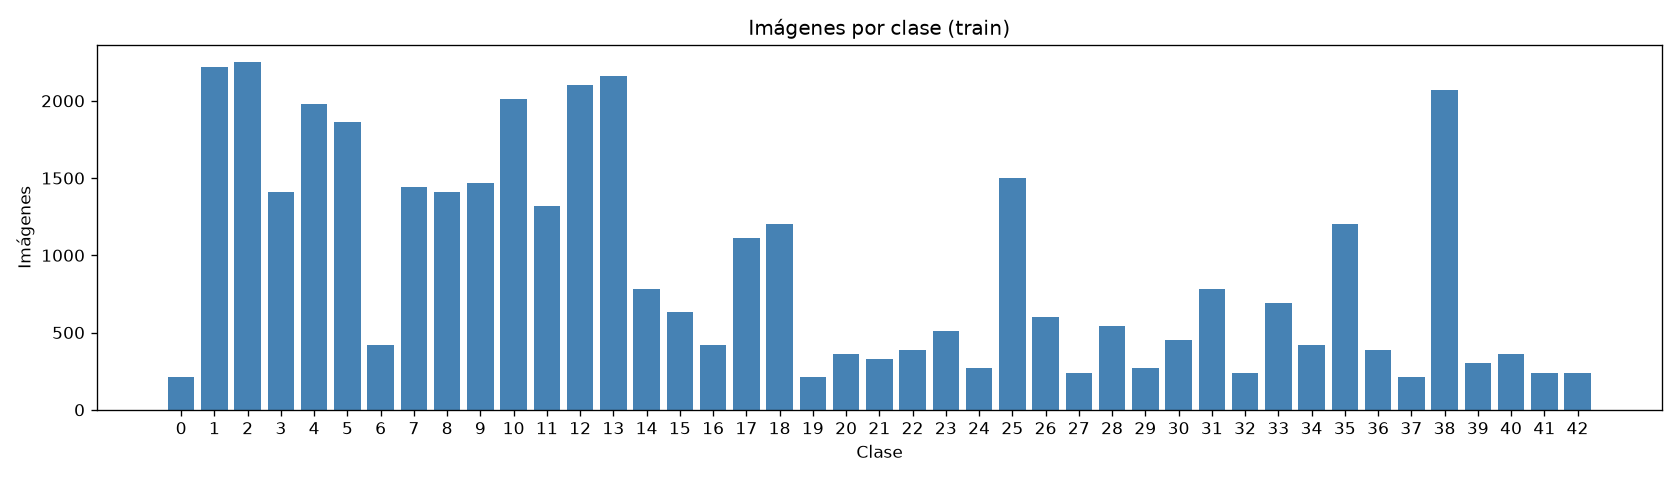
\includegraphics[width=\textwidth]{eda_clases.png}
    \caption{Cantidad de im\'agenes por clase en el conjunto de entrenamiento.}
    \label{fig:clases}
\end{figure}

Cada se\~nal f\'isica fue fotografiada en una secuencia o \emph{track} mientras el veh\'iculo se aproximaba. Las im\'agenes consecutivas son casi id\'enticas; una divisi\'on aleatoria por imagen colocar\'ia ejemplos del mismo objeto en entrenamiento y validaci\'on. Para evitar una estimaci\'on optimista, los 1,307 tracks se dividieron de forma estratificada: 33,299 im\'agenes para entrenamiento y 5,910 para validaci\'on, sin tracks compartidos. El test oficial se reserv\'o para la comparaci\'on final.

\begin{figure}[H]
    \centering
    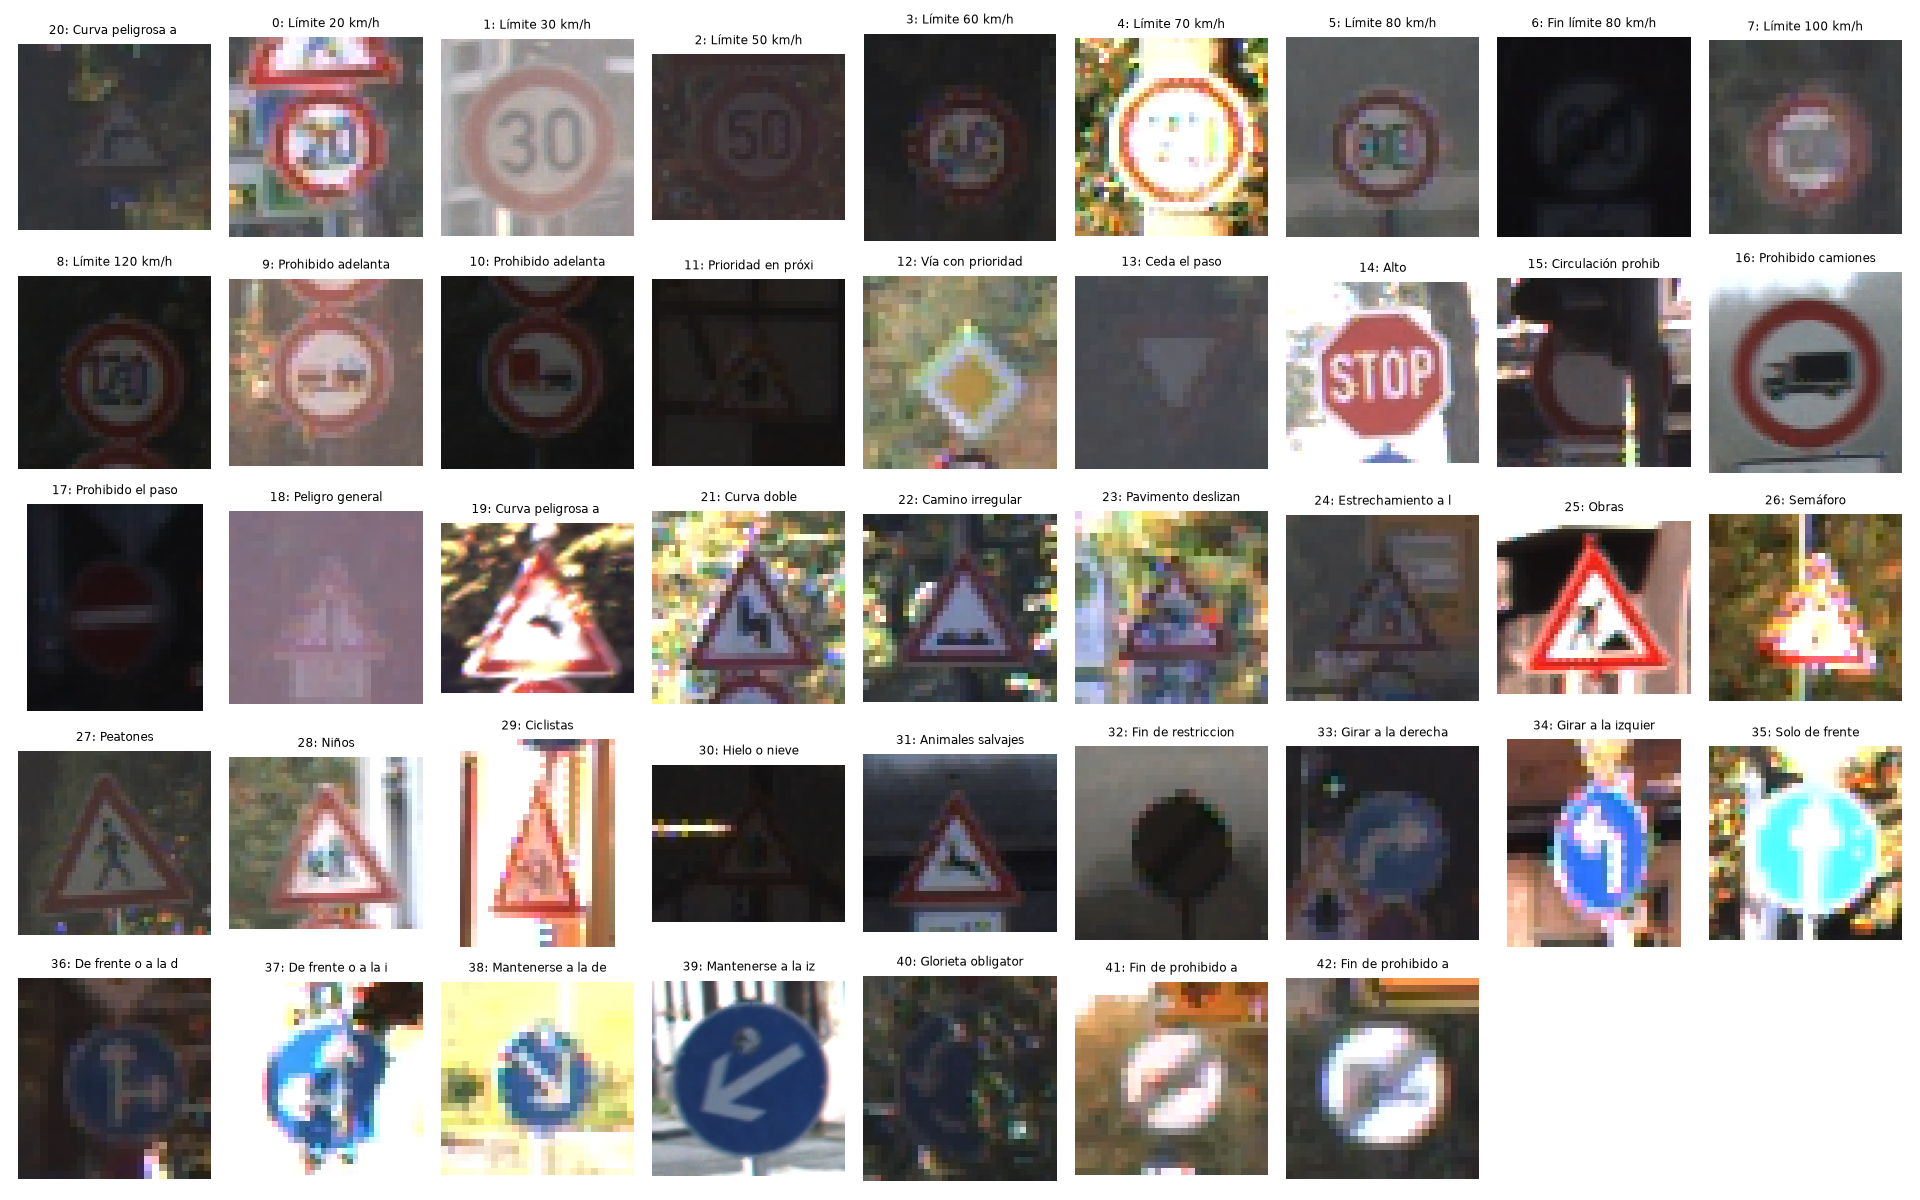
\includegraphics[width=0.96\textwidth]{eda_ejemplos.png}
    \caption{Ejemplo de cada una de las 43 clases de GTSRB.}
    \label{fig:ejemplos}
\end{figure}

\section{Propuesta de soluci\'on}

Se propuso comparar una arquitectura especializada y compacta con un modelo preentrenado de uso general. La CNN propia procesa im\'agenes de $48\times48$ p\'ixeles. MobileNetV2 utiliza entradas de $96\times96$ para reducir el costo en CPU, manteniendo la normalizaci\'on de ImageNet. En ambos casos se aplican rotaciones peque\~nas, traslaci\'on, cambios de escala, brillo, contraste y saturaci\'on durante entrenamiento. No se utiliza reflexi\'on horizontal porque alterar\'ia el significado de se\~nales direccionales.

El flujo completo comprende descarga y validaci\'on de datos, entrenamiento, selecci\'on mediante p\'erdida de validaci\'on, evaluaci\'on en el test oficial, an\'alisis de errores, robustez, explicabilidad e inferencia interactiva. Todos los experimentos usan semilla 42 y conservan los pesos de la mejor \`epoca mediante \emph{early stopping}.

\section{Descripci\'on de la soluci\'on}

\subsection{CNN desde cero}

La red propia contiene tres bloques convolucionales con 32, 64 y 128 canales. Cada bloque aplica dos secuencias convoluci\'on--BatchNorm--ReLU, seguidas por max pooling y dropout espacial. Un pooling promedio global transforma los mapas finales en un vector de 128 componentes. El clasificador contiene una capa de 256 unidades, ReLU, dropout y una salida de 43 logits. La arquitectura tiene 331,531 par\'ametros entrenables.

El entrenamiento usa Adam con tasa inicial $10^{-3}$, reducci\'on de tasa ante estancamiento y paciencia de cinco \`epocas. La ejecuci\'on termin\'o por early stopping en la \`epoca 26; la menor p\'erdida de validaci\'on se obtuvo en la \`epoca 21.

\begin{figure}[H]
    \centering
    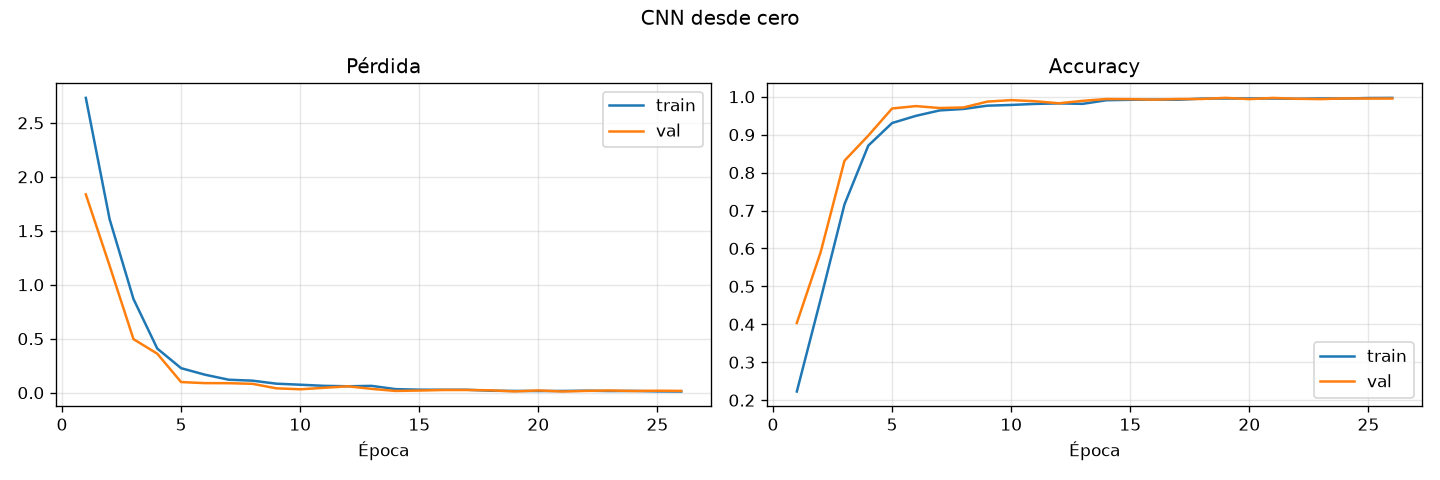
\includegraphics[width=\textwidth]{curvas_cnn.png}
    \caption{P\'erdida y exactitud durante el entrenamiento de la CNN.}
    \label{fig:curvas-cnn}
\end{figure}

\subsection{Transfer learning con MobileNetV2}

MobileNetV2 emplea convoluciones separables en profundidad y bloques residuales invertidos \cite{sandler2018}. En la etapa A se sustituy\'o el clasificador y se congel\'o el extractor preentrenado; solamente 55,083 par\'ametros (2.4\%) quedaron entrenables. En la etapa B se descongelaron los \`ultimos cuatro bloques y se usaron tasas de $10^{-4}$ para el backbone y $10^{-3}$ para el clasificador. Esta configuraci\'on elev\'o el n\'umero de par\'ametros entrenables a 1,581,163 (69.4\%).

\begin{figure}[H]
    \centering
    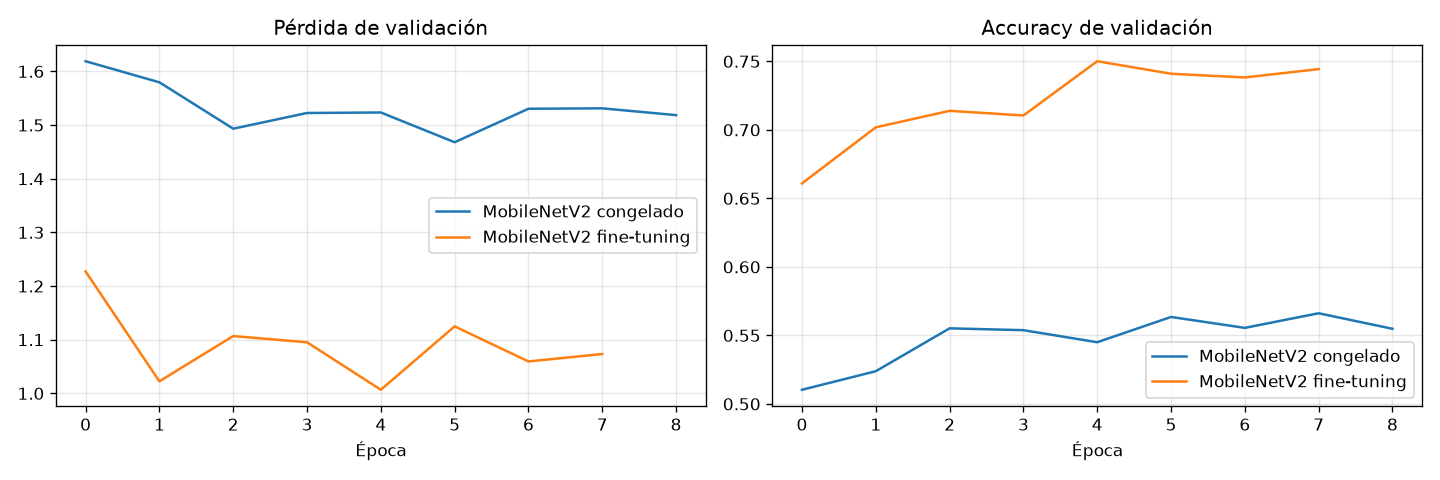
\includegraphics[width=\textwidth]{curvas_mobilenet.png}
    \caption{Comparaci\'on de las etapas de transferencia y ajuste fino.}
    \label{fig:curvas-mobile}
\end{figure}

\subsection{Inferencia y aplicaci\'on}

La l\'ogica de inferencia se separ\'o de los notebooks en un m\'odulo que carga el checkpoint, reproduce la transformaci\'on de evaluaci\'on y devuelve las cinco clases de mayor probabilidad. La interfaz Gradio permite cargar una imagen, consultar las probabilidades y visualizar la explicaci\'on Grad-CAM. El sistema se ejecuta localmente en CPU y no necesita acceso a servicios externos una vez instaladas las dependencias y descargado el modelo.

\section{Herramientas aplicadas}

La implementaci\'on utiliza Python, PyTorch y torchvision para modelos y entrenamiento; pandas y NumPy para manipulaci\'on de datos; scikit-learn para m\'etricas; Pillow y OpenCV para im\'agenes; Matplotlib y seaborn para visualizaci\'on; kagglehub para obtener el conjunto de datos; y Gradio para la demostraci\'on interactiva. Los notebooks documentan las decisiones experimentales y los m\'odulos de \texttt{src/} concentran la l\'ogica reutilizable.

\subsection{Uso de herramientas de asistencia generativa}

Se utiliz\'o asistencia generativa durante la planificaci\'on, revisi\'on del enunciado, depuraci\'on del entorno y estructuraci\'on de m\'odulos. Sus respuestas se trataron como propuestas sujetas a verificaci\'on: los modelos fueron entrenados localmente, las m\'etricas se recalcularon sobre el test oficial, las funciones nuevas cuentan con pruebas y las figuras se inspeccionaron antes de incorporarlas. El historial resumido de solicitudes, resultados, errores y decisiones se conserva en \texttt{docs/prompts\_ia.md}. Entre los problemas identificados estuvieron dependencias ausentes, restricciones temporales de red y el manejo de procesos de carga en Windows. Esta revisi\'on permiti\'o distinguir errores de entorno de errores del modelo y mantener trazabilidad sobre la evoluci\'on de la soluci\'on.

\section{Resultados}

\subsection{Comparaci\'on global}

La Tabla~\ref{tab:resultados} resume la evaluaci\'on de las 12,630 im\'agenes del test oficial. La CNN supera a MobileNetV2 ajustada por 22.42 puntos porcentuales de exactitud y a la versi\'on congelada por 39.27 puntos. La cercan\'ia entre F1 macro y ponderado de la CNN muestra que el desempe\~no no se concentra solamente en las clases frecuentes.

\begin{table}[H]
    \centering
    \caption{Resultados sobre el test oficial de GTSRB.}
    \label{tab:resultados}
    \begin{tabular}{lrrrr}
        \toprule
        Modelo & Accuracy & F1 macro & F1 ponderado & ms/imagen \\
        \midrule
        CNN desde cero & \textbf{0.9918} & \textbf{0.9870} & \textbf{0.9919} & 7.41 \\
        MobileNetV2 congelada & 0.5991 & 0.5164 & 0.5962 & \textbf{3.09} \\
        MobileNetV2 fine-tuning & 0.7676 & 0.7102 & 0.7668 & 3.62 \\
        \bottomrule
    \end{tabular}
\end{table}

El resultado ilustra que transfer learning no garantiza una mejora. ImageNet contiene fotograf\'ias naturales a mayor resoluci\'on, mientras que GTSRB contiene objetos peque\~nos, centrados y con patrones geom\'etricos espec\'ificos. El ajuste fino mejora MobileNetV2 en 16.85 puntos de exactitud, pero la arquitectura especializada sigue siendo superior.

\begin{figure}[H]
    \centering
    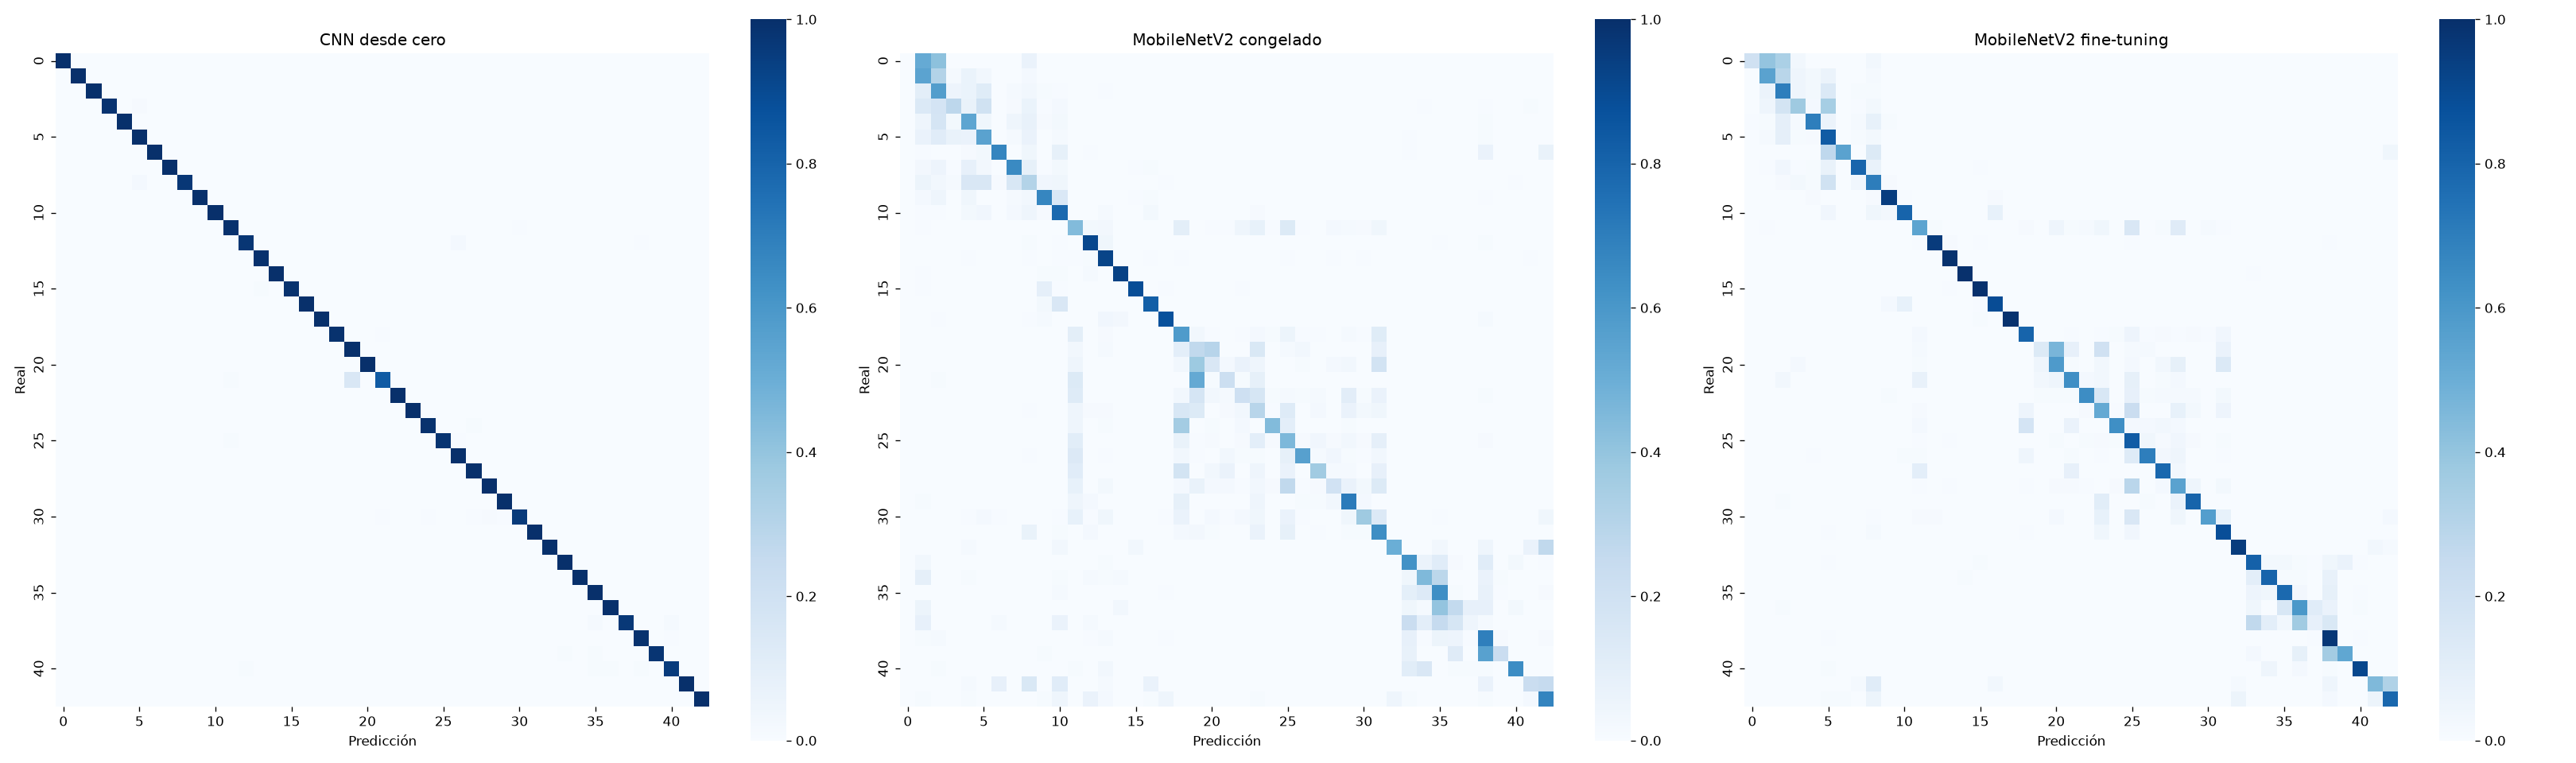
\includegraphics[width=\textwidth]{confusion_test.png}
    \caption{Matrices de confusi\'on normalizadas por clase.}
    \label{fig:confusion}
\end{figure}

\subsection{An\'alisis de errores}

La CNN comete pocos errores. Los pares m\'as frecuentes incluyen curva doble confundida con curva peligrosa a la izquierda (14 casos), v\'ia con prioridad confundida con sem\'aforo (14 casos) y l\'imite de 120 km/h confundido con 80 km/h (9 casos). MobileNetV2 concentra muchos errores en l\'imites de velocidad: por ejemplo, la versi\'on ajustada confunde 209 im\'agenes de 30 km/h con 50 km/h y 157 im\'agenes de 60 km/h con 80 km/h. Estas clases comparten forma circular, borde rojo y d\'igitos que pueden perder detalle al reducir la resoluci\'on.

\subsection{Robustez}

La CNN seleccionada se evalu\'o sin reentrenamiento bajo tres perturbaciones y tres severidades. El brillo se multiplic\'o por 0.78, 0.56 y 0.34; el ruido gaussiano utiliz\'o desviaciones est\'andar de 0.045, 0.090 y 0.135 sobre intensidades normalizadas; y el desenfoque gaussiano us\'o radios de 0.8, 1.6 y 2.4 p\'ixeles.

\begin{table}[H]
    \centering
    \caption{Accuracy de la CNN por perturbaci\'on y severidad.}
    \label{tab:robustez}
    \begin{tabular}{lrrrr}
        \toprule
        Condici\'on & Nivel 0 & Nivel 1 & Nivel 2 & Nivel 3 \\
        \midrule
        Brillo reducido & 0.9918 & 0.9914 & 0.9872 & 0.9815 \\
        Ruido gaussiano & 0.9918 & 0.9569 & 0.8359 & 0.7188 \\
        Desenfoque gaussiano & 0.9918 & 0.9816 & 0.8344 & 0.5574 \\
        \bottomrule
    \end{tabular}
\end{table}

\begin{figure}[H]
    \centering
    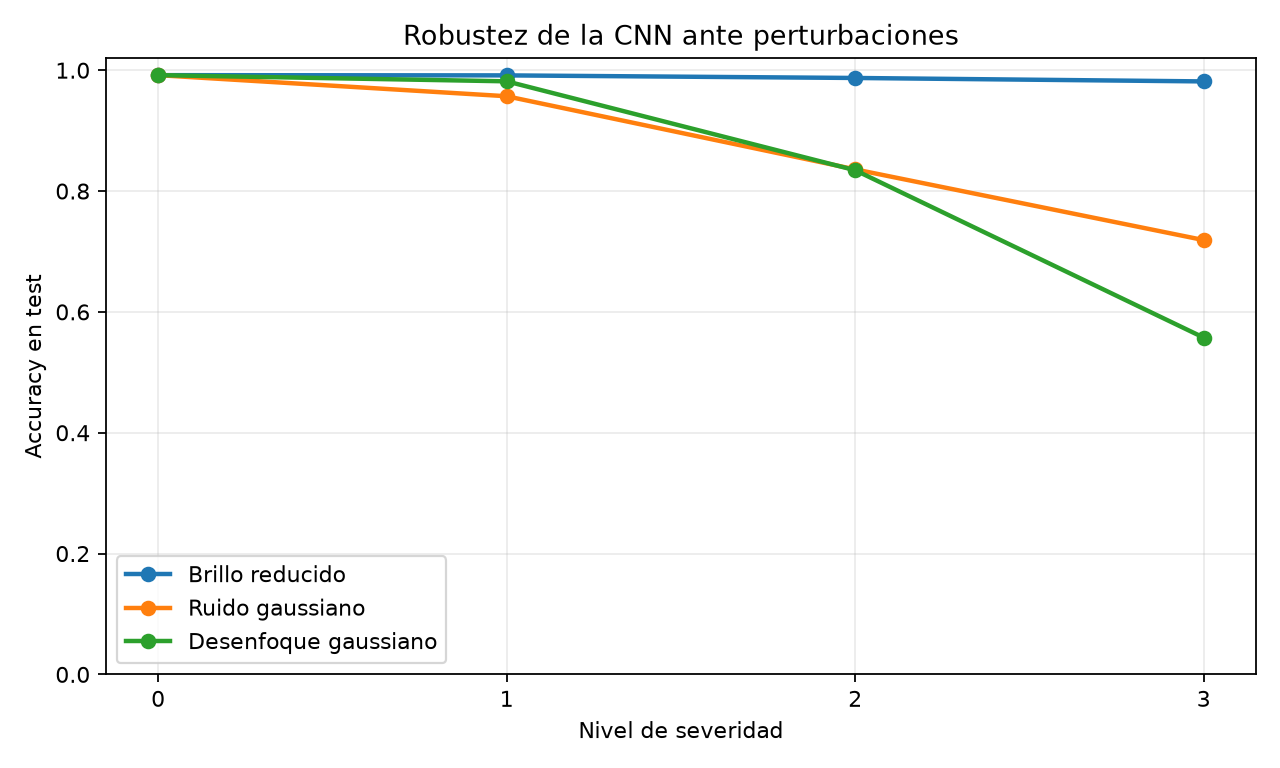
\includegraphics[width=0.85\textwidth]{robustez_curvas.png}
    \caption{Degradaci\'on de accuracy conforme aumenta la severidad.}
    \label{fig:robustez}
\end{figure}

El oscurecimiento tiene un efecto limitado: incluso en el nivel 3 la exactitud permanece en 98.15\%. El ruido y el desenfoque producen degradaciones no lineales. El desenfoque severo reduce la exactitud a 55.74\%, el peor resultado observado, porque elimina bordes y d\'igitos esenciales para separar clases similares. Este resultado sugiere que una versi\'on futura debe incluir desenfoque y ruido en el aumento de datos.

\subsection{Explicabilidad con Grad-CAM}

Grad-CAM pondera los mapas de activaci\'on de la \`ultima capa convolucional mediante los gradientes de la clase seleccionada \cite{selvaraju2017}. Los mapas muestran que en los aciertos la red concentra su respuesta en el interior de la se\~nal y en sus s\'imbolos. En los errores tambi\'en localiza la se\~nal, pero atiende regiones degradadas o insuficientes para distinguir detalles de clase. Por tanto, la mayor parte de los fallos analizados corresponde a clasificaci\'on fina y no a una atenci\'on completamente desviada hacia el fondo.

\begin{figure}[H]
    \centering
    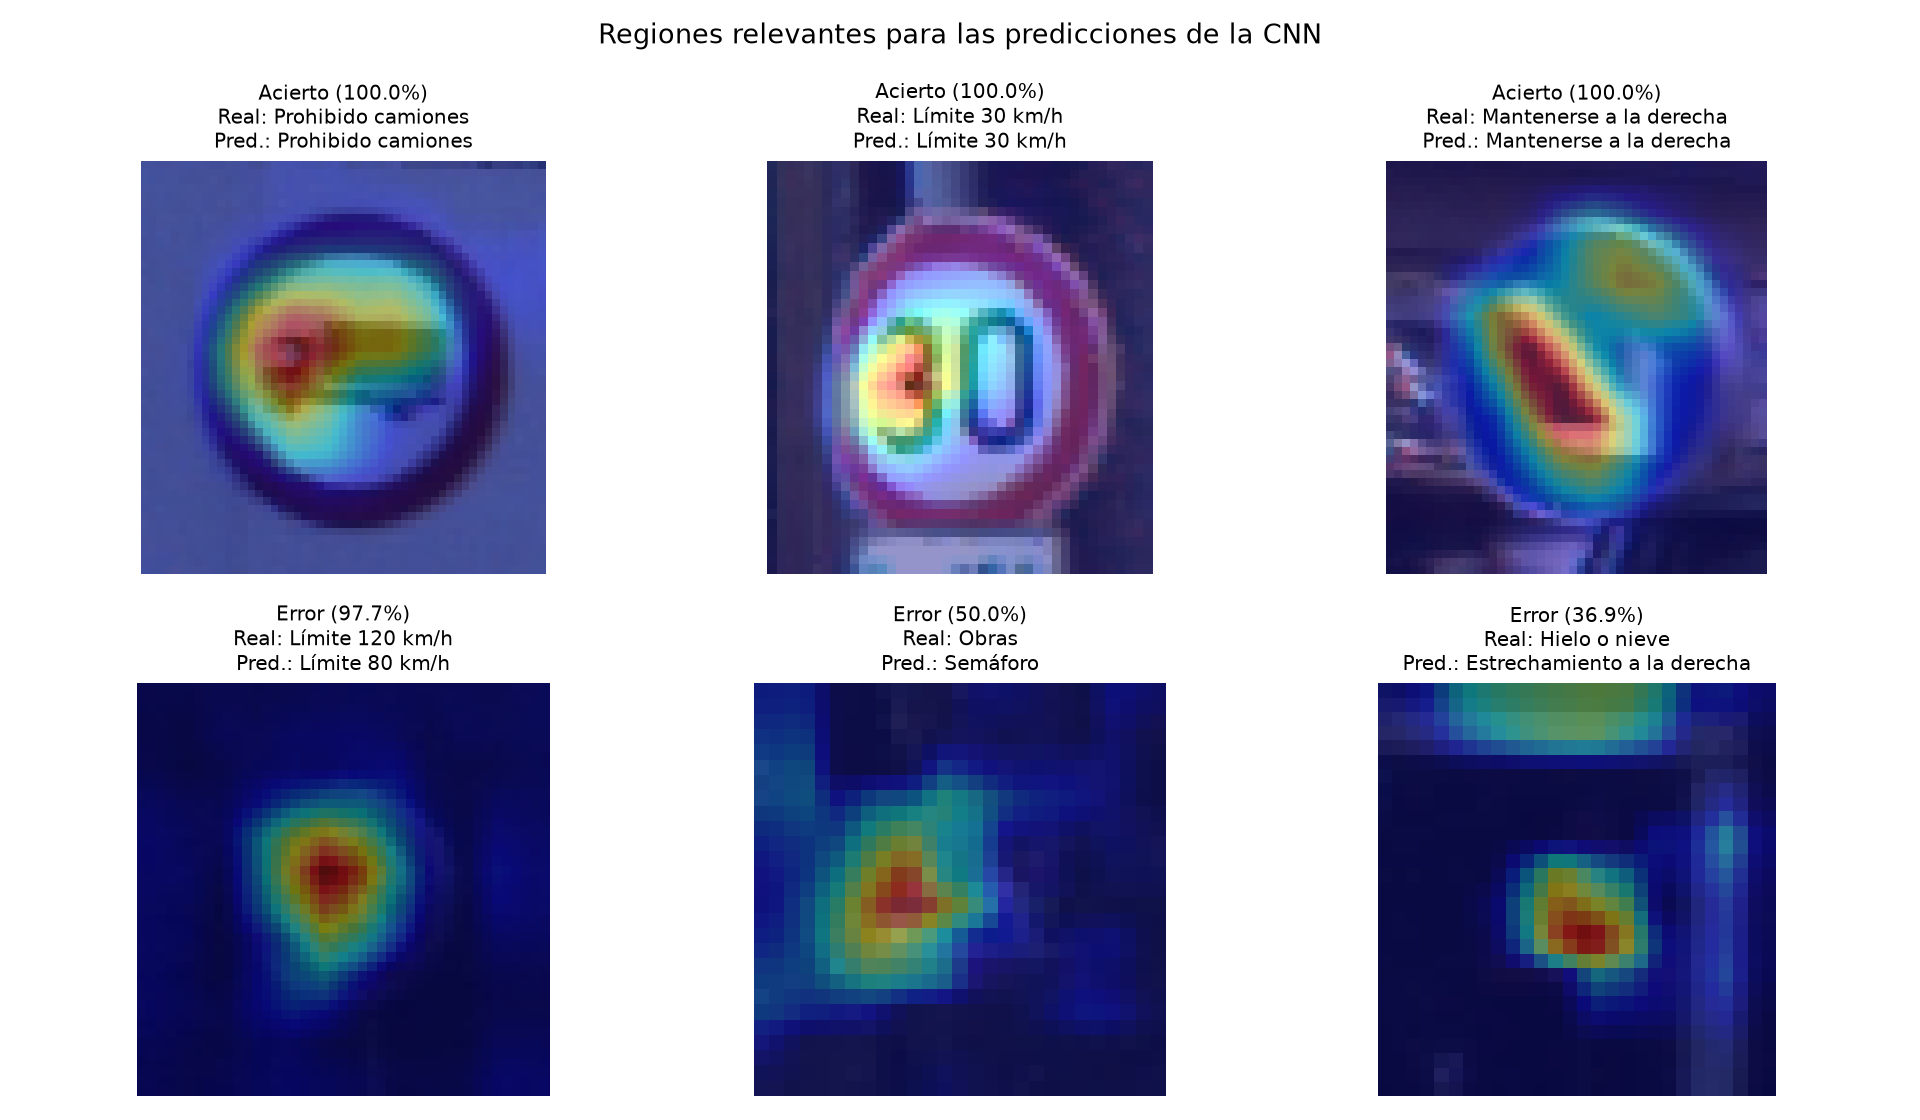
\includegraphics[width=\textwidth]{gradcam_ejemplos.png}
    \caption{Grad-CAM en tres aciertos (fila superior) y tres errores (fila inferior).}
    \label{fig:gradcam}
\end{figure}

\section{Limitaciones}

Los tiempos se midieron en CPU y dependen del equipo, tama\~no de lote y sistema de entrada/salida. MobileNetV2 se evalu\'o a $96\times96$ y no a la resoluci\'on habitual de ImageNet, lo que reduce costo pero puede limitar la transferencia. La robustez considera perturbaciones sint\'eticas aisladas; no representa todas las combinaciones de clima, movimiento, oclusi\'on y perspectiva del mundo real. Grad-CAM ofrece una explicaci\'on espacial aproximada y no demuestra causalidad. Finalmente, GTSRB corresponde a se\~nales alemanas y no cubre todas las variantes regionales.

\section{Conclusiones}

La CNN compacta entrenada desde cero fue la mejor alternativa para GTSRB: alcanz\'o 99.18\% de exactitud y 98.70\% de F1 macro, con un costo de 7.41 ms por imagen en CPU. MobileNetV2 mejor\'o sustancialmente mediante fine-tuning, pero sus caracter\'isticas preentrenadas no igualaron a la arquitectura especializada. La separaci\'on por tracks, el uso de m\'etricas macro y el test oficial permiten sostener que el resultado no depende de fuga entre secuencias ni solamente de clases frecuentes.

El an\'alisis de robustez identific\'o el desenfoque como la principal debilidad: la exactitud cae a 55.74\% en la severidad m\'axima, mientras que el oscurecimiento severo conserva 98.15\%. Grad-CAM confirma que la red suele atender la regi\'on de la se\~nal incluso cuando se equivoca. Como continuaci\'on se propone entrenar con ruido y desenfoque, calibrar las probabilidades, evaluar im\'agenes locales y ampliar el conjunto con se\~nales de otras regiones.

\section*{Video de demostraci\'on}
\addcontentsline{toc}{section}{Video de demostraci\'on}

El video muestra la aplicaci\'on Gradio clasificando se\~nales en vivo con su explicaci\'on Grad-CAM, describe brevemente la implementaci\'on y resume los hallazgos principales. Est\'a disponible en: \url{\videourl}

\section*{Reproducibilidad}
\addcontentsline{toc}{section}{Reproducibilidad}

Repositorio p\'ublico: \url{https://github.com/tismajo/CC2017-ProyectoFinal}

El repositorio contiene los m\'odulos de datos, modelos, entrenamiento, m\'etricas, inferencia, robustez y Grad-CAM; notebooks ejecutados; scripts para regenerar figuras; pruebas automatizadas; y la aplicaci\'on Gradio. El archivo \texttt{requirements.txt} enumera las dependencias. El dataset se almacena en la cach\'e de kagglehub y no se duplica en el repositorio.

\begin{thebibliography}{9}
\bibitem{stallkamp2012}
J. Stallkamp, M. Schlipsing, J. Salmen y C. Igel,
``Man vs. computer: Benchmarking machine learning algorithms for traffic sign recognition'',
\emph{Neural Networks}, vol. 32, pp. 323--332, 2012.

\bibitem{sandler2018}
M. Sandler, A. Howard, M. Zhu, A. Zhmoginov y L.-C. Chen,
``MobileNetV2: Inverted residuals and linear bottlenecks'',
\emph{Proceedings of the IEEE Conference on Computer Vision and Pattern Recognition}, pp. 4510--4520, 2018.

\bibitem{selvaraju2017}
R. R. Selvaraju et al.,
``Grad-CAM: Visual explanations from deep networks via gradient-based localization'',
\emph{Proceedings of the IEEE International Conference on Computer Vision}, pp. 618--626, 2017.

\bibitem{pytorch}
A. Paszke et al.,
``PyTorch: An imperative style, high-performance deep learning library'',
\emph{Advances in Neural Information Processing Systems}, vol. 32, 2019.
\end{thebibliography}

\end{document}
